\textit{(                                                                                )}

\begin{lstlisting}
# 5. Architecture Integration

A major contribution of HIBA is its robust `copy_weights` procedure, designed to seamlessly inject into disparate transformer families without silent failures.

## 5.1 Nested Encoder Detection (RoBERTa / BERT)

RoBERTa's attention block wraps the self-attention mechanism in an outer `BertSelfOutput` class that applies the final dense projection:

\end{lstlisting}
\section{HIBA Auto-Detection Logic}
if hasattr(pretrained\_attn, "self") and hasattr(pretrained\_attn.self, "query"):
    self.is\_nested\_encoder = True

\begin{lstlisting}

When `is_nested_encoder` is True, HIBA intercepts the forward pass *before* `self.out_proj` is applied, preventing severe signal attenuation caused by double-projection. The base weights for `W_q, W_k, W_v` are extracted deeply from `pretrained_attn.self`.

## 5.2 Fused Conv1D Handling (GPT-2)

GPT-2 stores $Q,K,V$ weights as a single fused `Conv1D` tensor with transposed dimensions $(d, 3d)$. HIBA detects this, transposes the weights to standard linear layout $(3d, d)$, and strictly chunks them:

\end{lstlisting}
c\_w = c\_w.t()
split\_size = c\_w.size(0) // 3
extracted["q"] = c\_w[:split\_size, :]
extracted["k"] = c\_w[split\_size : 2 * split\_size, :]
\section{...}

\begin{lstlisting}

## 5.3 Modern Architectural Features

* **Grouped-Query Attention (GQA):** HIBA natively checks if `num_kv_heads < num_heads` and dynamically applies `repeat_kv` during the forward pass, ensuring compatibility with Qwen, LLaMA, and Mistral.
* **Rotary Position Embeddings (RoPE):** HIBA implements `apply_rotary_pos_emb` with partial dimension rotation. It rotates only the first `rotary_dim` coordinates and concatenates the unrotated pass-through coordinates, perfectly matching Qwen3.5's behavior (e.g., `head_dim=256, rotary_dim=64`).
* **Strict Causality:** Causal masks are natively applied in both intra-block, inter-block, and rectification branches if `is_decoder=True`.

\end{lstlisting}



\begin{figure}[H]
\centering
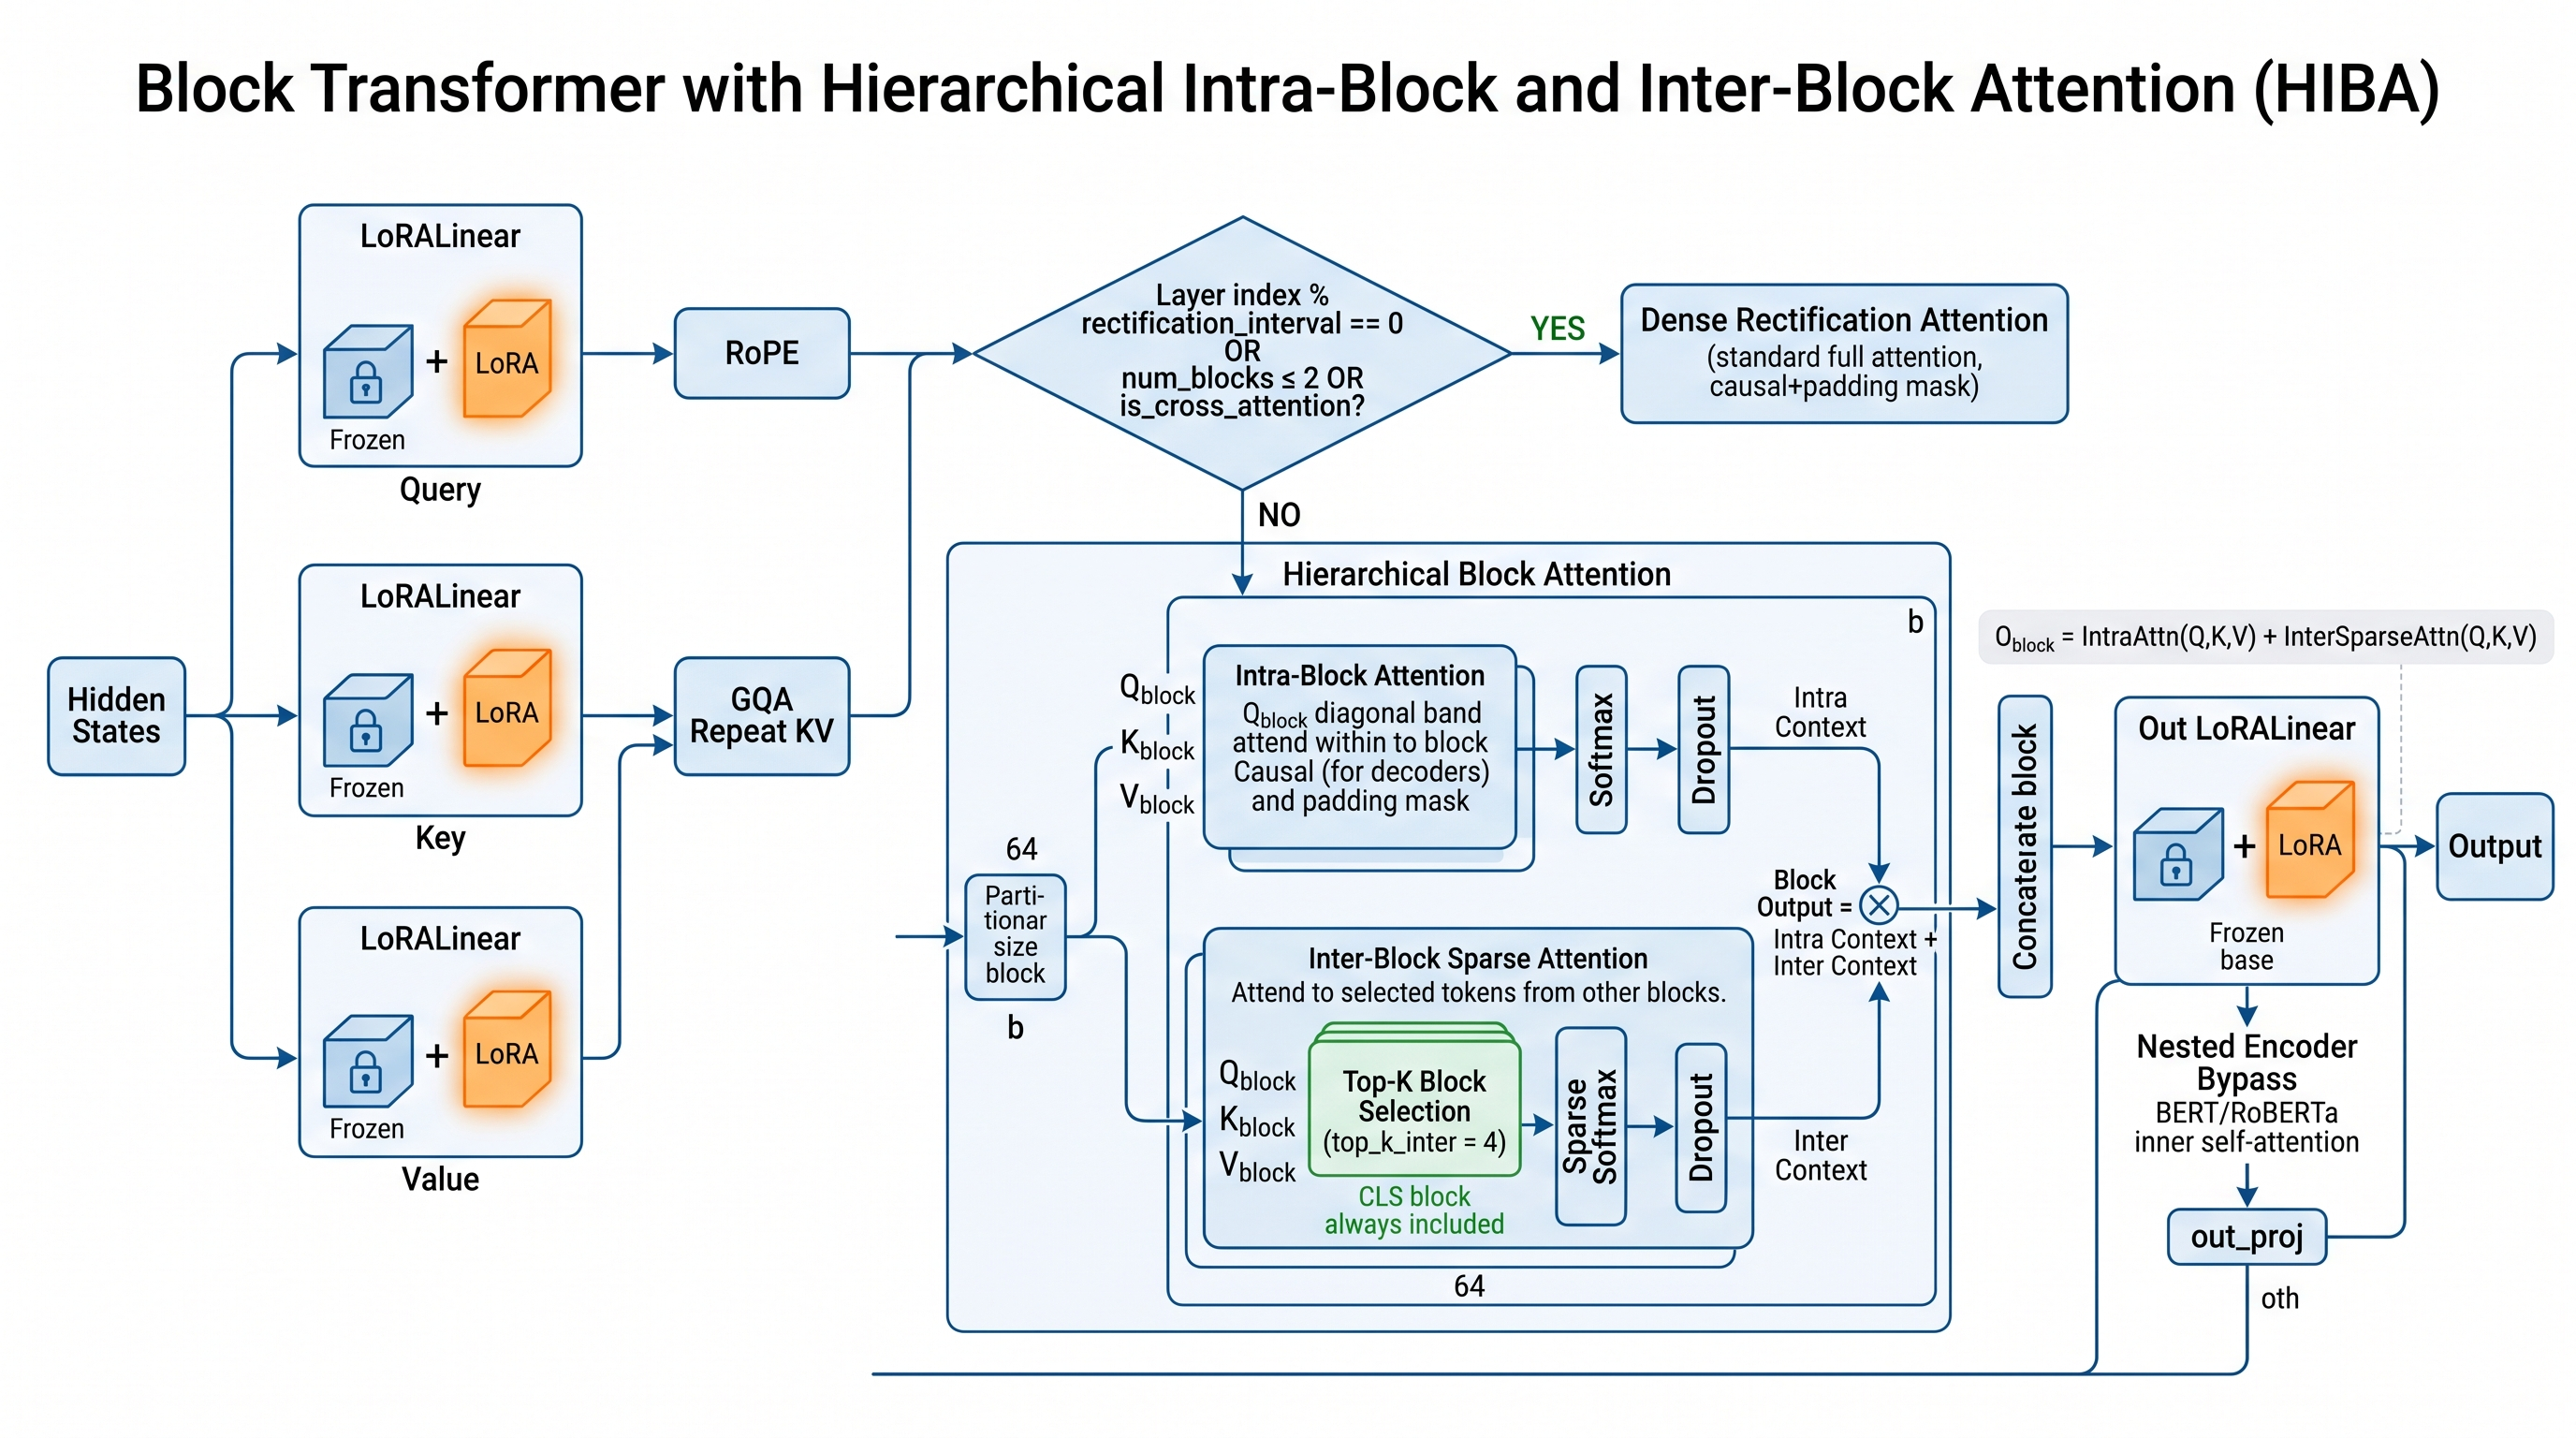
\includegraphics[width=\linewidth]{figures/architecture.jpeg}
\caption{High-level architectural diagram of block\_transformer\_hiba.}
\label{fig:arch_block-transformer-hiba}
\end{figure}

